\chapter{Compressive CRN Processing} 
\label{C:csp_css}

\indent \indent In the last chapter \ref{C:wideband_css}, we have discussed the main drawback in compressed sensing based spectrum sensing (CS-CSS) which derives from the computational non-linear CS reconstruction. As a fact, the CS framework sacrifices the time and energy performance in reconstruction produce (in return, the sampling rate is reduced). In order to solve this problem, this chapter focuses on exploring the potential approach of directly analysing compressive measurements without fully CS reconstruction. The new approach is termed as compressive signal processing (CSP), and it will be used for compressive spectrum sensing (CSS) in cognitive radio network (CRN), so that the drawback will be overcome. 

\section{Introduction}

\indent \indent The compressed sensing based wideband spectrum sensing for cognitive radio provides its outstanding feature in reducing the sampling rate. However, the corresponding drawbacks emerge in real-time ability and energy cost, mainly due to its computational complex non-linear reconstruction and energy cost in entire cognitive radio systems.  

However, many signal processing applications such as detection, classification, estimation and filtering do NOT require entire signal reconstruction \cite{davenport2010signal}. For instance, cognitive radios are aiming at processing the hypothesis detection rather than fully recovering the primary signals. In these cases, the aim of CS fully recovery is no longer necessary, so processing schemes like 'directly analysis without recovery' or 'partial recovery then analysis' become possible and applicable for cognitive spectrum sensing. 

This novel idea derives from the compressive signal processing (CSP)\cite{davenport2010signal}, which aims at extracting information directly from compressive samples without fully recovery. Further, this idea is developed in both theory and applications. In \cite{ohlsson2013compressive}, the shift retrieval problem for compressive samples is researched. Rather than recovering CS data then analysing the shifted distance, the author develops efficient algorithms and proofs for directly recognising the shift distance from CS data. Valsesia et al \cite{valsesia2014compressive} develops the circulant sensing matrix based processing for compressive measurements, which displays an potential CSP application for convolution based models and is suitable for filtering or channel impulse response involved cases. Especially, for cognitive radio spectrum detection, a CSP based energy detector is designed in \cite{appaiah2013spectrum}. Further, Guo et al develops CSP for feature detector in \cite{guo2013feature} and pattern clustering is achieved.

Since the paper \cite{guo2013feature} in year 2013 GLOBECOM conference says, "So far the CSP concept is only defined in the theory level and has not been applied to CR field", we believe there still exists many worthy research area and cases for CSP based CR spectrum sensing. In conclusion, CSP based cognitive spectrum sensing is still a relative new approach which applies the CS but throw away some CS drawbacks for CR specrum sensing. The following sections are organised as different function introduction for CSP based cognitive radio spectrum sensing, including filtering, detection, estimation. Some related potential application for CS-UWB and CS demodulation are also introduced.

\section{CSP Filtering for Cognitive Spectrum Sensing}\label{sct:csp_filter}
\indent \indent In scenarios where cognitive spectrum sensing requires filters, the design cost for analog filters are expensive. Then we can use CSP based filtering to transform the analog filter to digital filter, which omits the implementation of hardware design for filters.

\paragraph{Filter domain transform}
Assume that the filter's impulse response is $h$ (with length of $N_h$) and its corresponding matrix form is $H$, then $H$ is a circulant sensing matrix. Then, according to a CSP related theory in \cite{valsesia2014compressive}, it possible to exchange the $H$ and $\Phi$ (compressed sensing matrix), transform the analog filter into digital domain for filters within CS frameworks. In other words, the compressive measurements $y$ can be directly processed by filtering $H$ without recovery in some cases \ref{csp-filter} as follows:  
\begin{equation}
\label{csp-filter}
\hat y = \Phi H x = H \Phi x = H y \quad, where \quad i \in [1,m-N_h+1].
\end{equation}
, where the $\Phi$ is compressed sensing matrix with size of $m \times N$.  Consequently, by moving the filtering from analog to digital part, large amount of hardware complexity is omitted. 

\begin{figure}[!t]
\centering
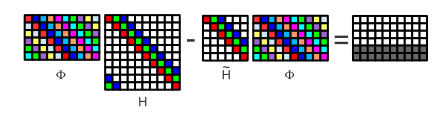
\includegraphics[width=5.0in]{figs/csp-filter-thm.png}
\DeclareGraphicsExtensions.
\caption{Block diagram of exchanging order of circulant matrix. $H$ is corresponding impulse response of filter, $\Phi$ is the compressed sensing matrix. The exchanging sacrifice is the loss of rows in the results (matrix in the right side of equal sign).}\label{csp-filter-thm}
\end{figure}

\paragraph{Interference filtering}
In cases where useless information is redundancy for further recovery in CS framework, or specifically where some sub-bands are priorly known in the compressive cognitive spectrum sensing, system using CSP can regard those useless information as interference and apply CSP-filtering to sample-then-filter the compressive data rather than sample-recover-then-filter it. 

Assume a sparse signal $x \in R^N$ which consists of two components:
\begin{equation}
\label{csp1}
x = x_s + x_I, \quad x_S \in S_S\; and\; x_I \in S_I
\end{equation}
, where the $x_S$ contains the spectrum of interest and the $x_I$ stands for the useless information. After the CS acquisition, we gain $y = \Phi x = \Phi(x_S + x_I)$. Then our aim is to wipe out the contribution of $\Phi x_I$ from the observation $y$ before recovering $x$. The following theorem provide the applicability of this idea:  
\begin{theorem}\cite{davenport2010signal}
\label{csp2}
Suppose that $\Phi$ satisfies the $\delta$-stable RIP for all $x_S\in\Sigma_S$ and $x_I\in\Sigma_I$, where $I$ is a $K_I$ dimensional subspace of $R^{N}$. Assume that $\Psi_I$ is an matrix whose columns constructs an orthogonal basis for the $K_I$ dimensional subspace. Define the matrix $P_{\Omega} = \Phi\Psi_I(\Phi\Psi_I)^{\dagger}$ and $P_{\Omega^{\perp}} = I-P_{\Omega}$. For any $x \in \Sigma_S \cup \Sigma_I$, we regard $x = x_S + x_I$, where $x_S \in s_S$ and $x_I \in s_I$, then
\begin{equation}
\label{csp3}
P_{\Omega^{\perp}} \Phi x = P_{\Omega^{\perp}} \Phi \hat x ,\quad
\frac{\delta}{1-\delta} \leq \|P_{\Omega^{\perp}} \Phi \hat x\|_2 \leq 1 + \delta 
\end{equation}
\end{theorem}
The theorem \ref{csp2} proofs that there exists a matrix $P_{\Omega^{\perp}}$ which is nearly orthogonal to the useless information $x_I$ such that $P_{\Omega^{\perp}} x_I \approx 0$. Hence the matrix $P_{\Omega^{\perp}}$ is the filter for selecting the desired signal $x_S$. we can apply this theory to construct a $filtering matrix$ in CS acquisition model if the support of the $x_I$ is known. 

\section{CSP Detection for Cognitive Spectrum Sensing}\label{sct:csp_detect}
\begin{figure}[!t]
\centering
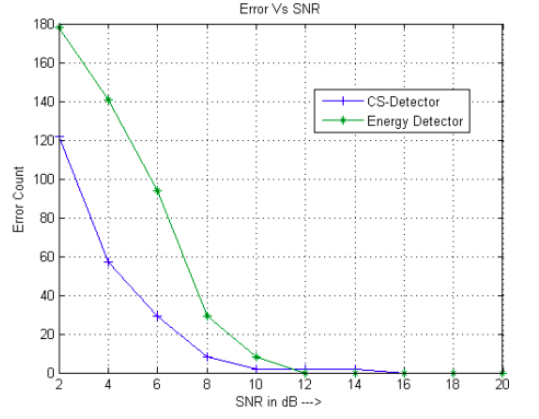
\includegraphics[width=4.0in]{figs/csp-detec_vs_ED.png}
\DeclareGraphicsExtensions.
\caption{Block diagram of performance comparison between the CSP detector (compressive signal processing based detector) and ED (energy detector) from aspect of signal to noise ratio and detection error.}\label{csp-detec_vs_ED}
\end{figure}

\paragraph{CSP based energy detector}
\indent \indent Davenport et al \cite{davenport2010signal} develops the theorem to directly build up hypothesis detection through compressed samples. Assume the detection is based on two hypotheses in 
\begin{equation}
\begin{aligned}
H0: y = \Phi w  \\
H1: y = \Phi (w + s)
\end{aligned}
\end{equation}
, where $s$ is the primary user's signal, $y$ is the vectorial observation, $\Phi$ is compressed sensing matrix (e.g. the random demodulation), and $w$ stands for the noise. Then the following equation \ref{csp-detect} presents the structure of CSP based detector. 
\begin{equation}
\label{csp-detect}
\Lambda(y) = (\Phi \Phi^T)^{-1} \Phi s \quad \mathop{\lessgtr}_{H_1}^{H_0} \quad \alpha
\end{equation}
In \cite{appaiah2013spectrum}, the experimental results of comparing CSP-detector and traditional energy detector (ED), which is shown in figure \ref{csp-detec_vs_ED}. One of the defect is that the theorem does not drive other blind sensing techniques for cases where the information of primary signal $s$ is unknown to us. Thus further developing for CSP based blind sensing is a potential direction. 

\paragraph{CSP based cyclic feature detector}
%re-write:
Guo et al develops CSP for feature detector in \cite{guo2013feature} and achieves pattern clustering.
The work generates the compressive CR spectrum measurement by utilizing both the cyclic-stationary feature and sparsity prior knowledge at the spectrum sensing front end. Then the paper applies the compressive CSP without the need of signal or feature reconstruction. However, as the author says in \cite{guo2013feature}, the CSP feature detection model is still simple. How to analyze the spectrum pattern recognition performance in a more complicated CRN environment is open issue. For instance, with large-scale SUs and non-Poisson PU traffic models. Also, More efficient machine learning schemes (such as information geometry) can be used to recognize the PUs’ signal patterns after obtaining the CS samples via CSP scheme. 

\section{CSP Estimation for Cognitive Spectrum Sensing}\label{sct:csp_estim}
\indent \indent  Since the signal-to-noise-ratio, sparsity order are crucial factors which seriously affects the performance of compressive detectors, CSP based estimation becomes popular for cognitive radio. This technique make CR predict the level of sparsity or noise, so that CR can vary the sampling rate or changing detection algorithms:

\paragraph{Sparsity order estimation}
For instance, the sparsity order of the spectrum occupancy is time-varying in CR networks. If CR intends fully exploit the CS framework, the sampling rate of CS receiver should keeping adjusting to sparsity orders. Then \cite{sharma2014compressive} develops an approach which analysis sparsity order through asymptotic eigenvalue probability distribution function (aepdf) from the covariance matrix of the compressively sampled primary signal. In details, the aepdf is related to the sparsity order via a lookup table in figure \ref{csp-soe}. 

\begin{figure}[!t]
\centering
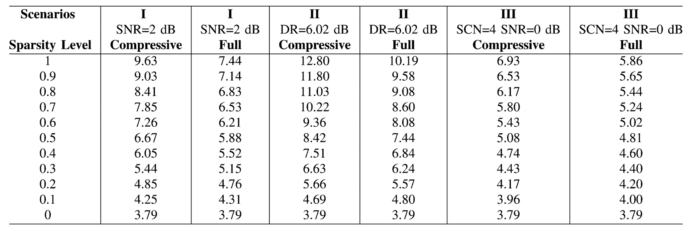
\includegraphics[width=4.0in]{figs/csp-soe.png}
\DeclareGraphicsExtensions.
\caption{Block diagram of lookup table for sparsity order estimation through signal-to-noise ratio (SNR) and asymptotic eigenvalue probability distribution function (aepdf). For example, if the value of aepdf = 7.26 for the compressive case in SNR = 2db, it can be estimated that the sparsity order of spectrum occupancy is 0.6}\label{csp-soe}
\end{figure}

\paragraph{Noise level estimation}
For CR networks, the signal-to-noise ratio (SNR) affects the performance of spectrum detectors. For example, the energy detector (ED) is simple and fast, but with poor performance in low SNR scenarios; Feature detectors (FD) are complex and slow, but have strong robustness to noise. In \cite{sharma2014compressive_snr}, the author similarily build up a lookup table relating the noise estimation with the eigenvalue probability distribution function in covariance matrix of the compressively sampled primary signal. 

\paragraph{Hybrid spectrum sensing} If we have known the SNR, we can design a more intelligent two stage detector. In the coarse stage, a quick search is done over a wide bandwidth, and in the fine stage, the sensing is done over the individual candidate sub-bands in that bandwidth, one at a time. the coarse stage is based on energy detection due to its fast processing. If the test statistics is larger than a predefined threshold, then the band is considered occupied. Otherwise, a fine stage is performed where a cycle-stationary detector is implemented due to its robustness at the low SNR regime. (For sparsity level, we can judge whether the CS based detector suitable if there exists dense channel occupancy by primary users)

\paragraph{Adaptive spectrum Sensing} In case when a CR successfully know the primary signals' SNR, the CR can intelligently choose optimal detection algorithms based on SNR related performance of detectors. For instance, if the SNR is detected to be very low, then cycle-stationary detection algorithm can be used due to its robustness at the low SNR regime. Otherwise, the energy detector can be used since it's fast and accurate enough in high SNR regime. Extending this idea of selecting various of detector based on CSP estimation, we can select the optimal detector adaptively. This will provide future cognitive radio more flexibility to the varying environment.

\section{Other Related Wideband Processing with CSP}

\subsection{CSP TOA Algorithm for Ultra-Wideband Positioning}\label{sct:csp_toa}
\indent \indent Maximizing the cross-correlation between the two signals is one of the key steps in time-of-arrival (TOA) algorithms which have been applied in compressive UWB positioning in chapter \ref{C:compressive_uwb_positioning}. In that system, the procedures at receiving end can be abstracted as (1) low-rate sampling, then (2) CS fully reconstruction, finally (3) TOA algorithm based locationing. However, the (2) CS fully reconstruction may sometimes Not necessary if we borrow the theorem in  \cite{ohlsson2013compressive}, where the shift retrieval problem for compressive samples is investigated. Rather than recovering CS data then analysing the shifted distance, the author develops efficient algorithms and proofs for directly recognising the shift distance from CS data. The paper illustrates the results by running a Monte Carlo simulation shown in figure \ref{csp-shift}. According to this result, the CSP-TOA positioning becomes possible.

\begin{figure}[!t]
\centering
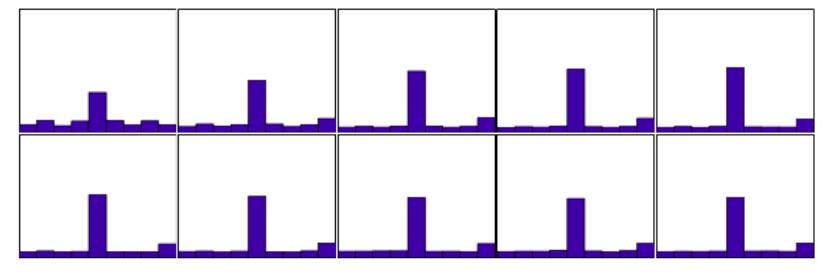
\includegraphics[width=5.0in]{figs/csp-shift.png}
\DeclareGraphicsExtensions.
\caption{Histogram for the estimated shift in SNR = 2. From left to right, top to bottom, compression ratio = 0.1 ... 1. The true shift was set to 5 in all trials}\label{csp-shift}
\end{figure}

\subsection{CSP Demodulation}
\indent \indent A compressive sensing phase-locked loop (CS-PLL) \cite{schnelle2012compressive}, is designed for directly extracting the phase and frequency from compressively sampled modulated signal $without$ sparse recovery. Since the restricted isometry property (RIP) of CS ensures that the standard inner product between $x[n]$ and $u[n]$ is approximately the same as that in the compressively sensed version produced by $y[m]$ and $u[n]$ \cite{davenport2010signal}, hence, the inner products in the standard PLL and that in the CS-PLL are nearly the same, ensuring the consistence between the standard PLL $\theta [n]$ and the CS-PLL's output $\theta [m]$. This idea is similar to the CSP estimation related theorem in section \ref{sct:csp_estim}. The presentation of the $\theta [m]$ can be presented as $\theta [m] = \sum_{k} y[k]v[k]h[m-k]$, where the index $m$ indicates the lower sampling rate compared with the Nyquist rate index $n$. In addition, the compressive sensing operations $\Phi$ which apply the RD's architecture consist of a input pseudo-random sequence, a mixer, a integrator, and a low-rate sampling ADC, which is the same as the RD's architecture shown in Figure \ref{RD}.

\begin{figure}[!t]
\centering
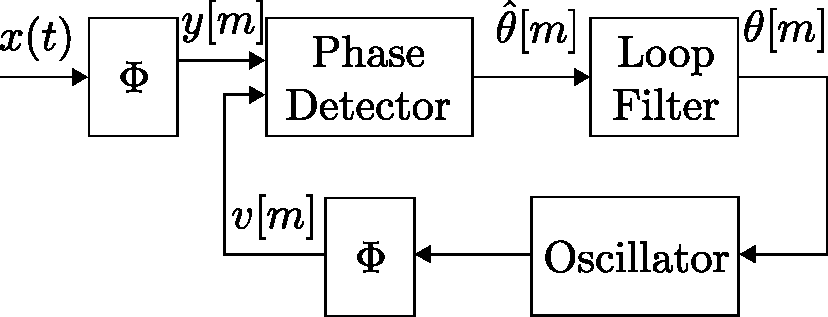
\includegraphics[width=2.6in]{figs/pll2.pdf}
\DeclareGraphicsExtensions.
\caption{Block diagram of the compressive sensing phase-locked loop (CS-PLL). The components includes the pre-CS sampler, phase detector, loop filter, oscillator and the feed-back CS multiplier}\label{CS-PLL}
\end{figure}

\section{Conclusion}

\indent \indent In the this chapter, we have followed the discussion of the main drawback in compressed sensing based spectrum sensing (CS-CSS) which derives from the computational non-linear CS reconstruction, and propose the idea of signal processing directly on compressively sampled data (CSP). Then we introduced our future potential works for cognitive spectrum sensing with CSP, including CSP filtering, CSP detection, CSP estimation. Also, potential CSP TOA Algorithm for Ultra-Wideband Positioning is introduced. We hope that by utilise the CSP in spectrum sensing, energy efficient hardware with high flexibility can be achieved in the future. 

%--------------------------------------------------------------

%As a fact, the CS framework sacrifices the time and energy performance in reconstruction produce (in return, the sampling rate is reduced). In order to solve this problem, this chapter focuses on exploring the potential approach of directly analysing compressive measurements without fully CS reconstruction. The new approach is termed as compressive signal processing (CSP), and it will be used for compressive spectrum sensing (CSS) in cognitive radio (CR), so that the drawback will be overcome. 

%In conclusion, the motivations for developing signal processing for compressed measurements can be categorised in following aspects:

%\paragraph{Demand for simple signal processing in CS}
%The reconstruction algorithms for CS is non-linear, which indicates that the recovered data are not directly suitable for conventional digital signal processing where a simple recovery using cardinal sine (sinc) interpolation (linear process) is required. One solution is to sequentially achieve CS reconstruction and then process the recovered data, but it's too computational expensive.

%\paragraph{Requirement for energy efficiency in CS}

%The discussion in chapter \ref{C:wideband_css} stresses the main drawback in CS based cognitive spectrum sensing. which derives from the computational non-linear CS reconstruction.


% %--------------------------------------------------------------
% 
% \section{Interference Avoidance}
% 
% Assume a sparse signal $x \in R^N$ which consists of two components:
% \begin{equation}
% \label{csp1}
% x = x_s + x_I, \quad x_S \in S_S\; and\; x_I \in S_I
% \end{equation}
% , where the $x_S$ contains the spectrum of interest and the $x_I$ stands for the useless information. After the CS acquisition, we gain $y = \Phi x = \Phi(x_S + x_I)$. Then our aim is to wipe out the contribution of $\Phi x_I$ from the observation $y$ before recovering $x$. The following theorem provide the applicability of this idea:  
% \begin{theorem}\cite{davenport2010signal}
% \label{csp2}
% Suppose that $\Phi$ satisfies the $\delta$-stable RIP for all $x_S\in\Sigma_S$ and $x_I\in\Sigma_I$, where $I$ is a $K_I$ dimensional subspace of $R^{N}$. Assume that $\Psi_I$ is an matrix whose columns constructs an orthogonal basis for the $K_I$ dimensional subspace. Define the matrix $P_{\Omega} = \Phi\Psi_I(\Phi\Psi_I)^{\dagger}$ and $P_{\Omega^{\perp}} = I-P_{\Omega}$. For any $x \in \Sigma_S \cup \Sigma_I$, we regard $x = x_S + x_I$, where $x_S \in s_S$ and $x_I \in s_I$, then
% \begin{equation}
% \label{csp3}
% P_{\Omega^{\perp}} \Phi x = P_{\Omega^{\perp}} \Phi \hat x ,\quad
% \frac{\delta}{1-\delta} \leq \|P_{\Omega^{\perp}} \Phi \hat x\|_2 \leq 1 + \delta 
% \end{equation}
% \end{theorem}
% The theorem \ref{csp2} proofs that there exists a matrix $P_{\Omega^{\perp}}$ which is nearly orthogonal to the useless information $x_I$ such that $P_{\Omega^{\perp}} x_I \approx 0$. Hence the matrix $P_{\Omega^{\perp}}$ is the filter for selecting the desired signal $x_S$. we can apply this theory to construct a $filtering matrix$ in CS acquisition model if the support of the $x_I$ is known. 
% In addition, it also points out that $P_{\Omega^{\perp}}\Psi$ satisfies the $\delta/(1-\delta)$-stable RIP for all $x \in \Sigma_{S_S}$, indicating that this filtering matrix provide a stable recovery:  
% \begin{theorem}\cite{davenport2010signal}
% \label{csp4}
% Suppose that $\Phi$ satisfies the $\delta$-stable RIP for all $x_S\in\Sigma_S$ and $x_I\in\Sigma_I$, where $I$ is a $K_I$ dimensional subspace of $R^{N}$. Assume that $\Psi_I$ is an matrix whose columns constructs an orthogonal basis for the $K_I$ dimensional subspace. Define the matrix $P_{\Omega}$ and $P_{\Omega^{\perp}}$ as in the theorem \ref{csp2}. Then the $P_{\Omega^{\perp}}\Phi$ satisfies $\delta/(1-\delta)$-stable RIP for all $x_S \in \Sigma_S$ and $P_{\Omega}\Phi$ satisfies $\delta$-stable RIP for all $x_I \in \Sigma_I$.  
% \end{theorem}
% 
% 
% 
% \paragraph{Requirement for real time ability in CS}
% \section{Compressive Estimation}
% \subsection{Compressive Phase-Locked Loop}
% \indent \indent Since computationally expensive for accurate sparse recovery is relatively high which reduces the real-time processing ability of CS devices, a compressive sensing phase-locked loop (CS-PLL)  \cite{schnelle2012compressive}, is designed for directly extracting the phase and frequency from compressively sampled modulated signal $without$ sparse recovery. This novel architecture brings computational advantages that improves the real-time processing capability in CS devices such as FM receivers\cite{davenport2010wideband} and widely implemented in wireless communication. 
% 
% %It applies a revised PLL structure by adding two compressive sensing (CS) operations $\Phi$ to the original standard architecture of PLLs: one operation is the pre-CS sampler representing the random demodulator (RD) for modulated signal acquisition; another one is the feed-back multiplier which has the same structure as the first, which locates between the oscillator and the phase detector. Then the new architecture of the CS-PLL is shown in Figure \ref{CS-PLL}, comprised of a pre-CS sampler, phase detector, loop filter, oscillator and a feed-back CS multiplier.
% 
% \begin{figure}[!t]
% \centering
% 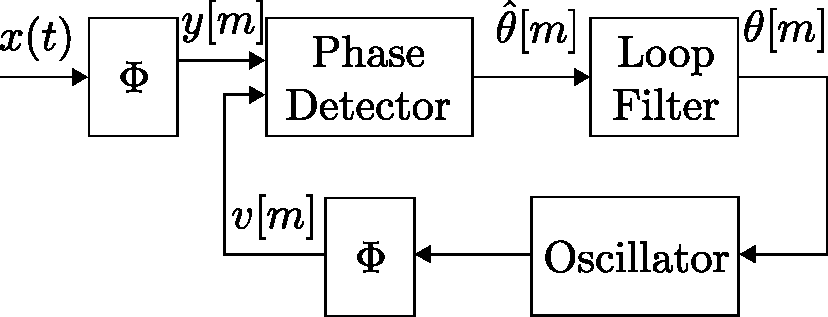
\includegraphics[width=2.2in]{figs/pll2.pdf}
% \DeclareGraphicsExtensions.
% \caption{Block diagram of the compressive sensing phase-locked loop (CS-PLL). The components includes the pre-CS sampler, phase detector, loop filter, oscillator and the feed-back CS multiplier}\label{CS-PLL}
% \end{figure}
% 
% Since the restricted isometry property (RIP) of CS ensures that the standard inner product between $x[n]$ and $u[n]$ is approximately the same as that in the compressively sensed version produced by $y[m]$ and $u[n]$\cite{davenport2010signal}, hence, the inner products in the standard PLL (\ref{eqn_pll1}) and that in the CS-PLL (\ref{eqn_pll2}) are nearly the same, ensuring the consistence between the standard PLL $\theta [n]$ and the CS-PLL's output $\theta [m]$. The presentation of the $\theta [m]$ can be presented as:
% \begin{equation}
% \label{eqn_pll2}
% \theta [m] = \sum_{k} y[k]v[k]h[m-k]
% \end{equation} 
% , where the index $m$ indicates the lower sampling rate compared with the Nyquist rate index $n$. In addition, the compressive sensing operations $\Phi$ which apply the RD's architecture consist of a input pseudo-random sequence, a mixer, a integrator, and a low-rate sampling ADC, which is the same as the RD's architecture shown in Figure \ref{RD}.
% 
%--------------------------------------------------------------

%\section{Compressive Sensing Processing} 

%\subsection{Applications: CSP Detector}

%\indent \indent the CSP-detector which estimates the existence of primary users directly from CS samples before recovery, so running time is significantly saved. Further, CS-filters, CS-estimators etc can also embedded for other scenarios in cognitive spectrum sensing, in order to improve the real-time capability direction, or further adaptive sensing schemes. Also, our future research direction will follow this idea.

%In this section, compressed sensing based spectrum sensing techniques for cognitive radio are introduced and compared. As a result, traditional sensing techniques of CR such as energy detector, feature detector can improve their detection performance if they implement the CS technique under the assumption that sensed spectrum are sparse. However, as the CS reconstruction requires non-linear processing which is much complex than traditional linear sinc based recovery, the real-time capability loss becomes the main payment for reducing the high sampling rate problem aforementioned in this chapter. Besides, the CS techniques highly relies on the assumption that object (spectrum) are sparse, in other words, CS is not  suitable for dense wireless communication environment. These two problems lead the following discussion in the next chapter, which shows our proposed research directions. 

%\section{Compressed Signal Processing for Cognitive Radio}\label{C:csp_cr}

%\indent \indent In aforementioned sections, compressed sensing based spectrum sensing techniques for cognitive radio are introduced and compared. As a result, traditional sensing techniques of CR such as energy detector (ED), coherent detector (CD) can improve their detection performance if they implement the CS technique under the assumption that sensed spectrum are sparse. However, as the CS reconstruction requires non-linear processing which is much complex than traditional linear sinc based recovery [xx-yy], the real-time capability loss becomes the main payment for reducing the high sampling rate problem aforementioned in this chapter. Besides, the CS techniques highly relies on the assumption that object (spectrum) are sparse, in other words, CS is not  suitable for dense wireless communication environment. These two problems lead the following discussion in the next chapter, which shows our proposed research directions. 

%\indent \indent In this chapter, we propose a potential approach, term as the compressive signal processing (CSP) [x], to enhance the real-time capability of compressed sensing based cognitive sensing framework under the assumption that in many cases fully recovery is NOT necessary. Followed by this idea, [xx-yy] successfully reduce the executive time since the magnitude of recovered signal length is significantly decreased. On the other hand, since cognitive spectrum sensing (CSS) only requires detecting the 'existence' of spectrum, so fine recovery is no need. From this aspect, the idea of CSP is well suited for CSS. In this chapter, an overview of the compressed signal processing (CSP) theory is presented, as well as the CSP-based applications in wireless communications. 

%\indent \indent In this chapter, we propose an overview of cognitive radio (CR) networks and then focus on the bottleneck in its front-end sampling devices. Due to the wideband sensing task in CR, the required sampling rate becomes extremely high. Although various approaches [xx-yy] are recently developed to solve this problem, it's shown that in many scenarios, the compressed sensing is the optimal method to solve the problem [xx-yy]. This chapter presents the recent work of compressed spectrum sensing for cognitive radio.

%-------------------------------------------------------------------------------------------------------------

%\section{Motivation}\label{sct:csp_moti}

%\indent \indent In the last chapter, compressed sensing based spectrum sensing techniques for cognitive radio are puzzled by the heavy burden from non-linear CS reconstruction procedure [xx-yy]. Previous approaches such as greedy recovery [xx-yy] aims at fast reconstruction while keeping considerable robustness, and they achieve to present enough contributions. 

%Besides, the CS techniques highly relies on the assumption that object (spectrum) are sparse, in other words, CS is not  suitable for dense wireless communication environment. These two problems lead the following discussion in the next chapter, which shows our proposed research directions. 

%--------------------------------------------------------------

%Besides, since accurate detection of cognitive spectrum sensing is always required for not interfering primary users, time consuming algorithms -- convex optimization (e.g.basis pursuit) is needed. In such cases, large delays are generated and in conflict with agility (i.e. feedback reconfiguration) in cognitive radios. 

%--------------------------------------------------------------

%However, in CS acquisition model, this relation no longer remains indicating we cannot directly achieve CS based signal processing without recovering the original data. What's worse, CS based reconstruction is always complicated than that in traditional Nyquist theory based ADCs: In traditional ADCs, signal reconstruction can be achieved by $sinc$ interpolation which is a linear processing with little computation, while the CS based signal reconstruction requires nonlinear computations such as convex optimization based or greedy pursuit algorithms, which are considered as  more computationally expensive\cite{davenport2010signal}. Therefore, the signal processing becomes a crucial problem in acquisition systems using CS based ADCs. 

%--------------------------------------------------------------

%Signal processing through compressive measurements is always difficult than that by traditional one. In traditional Nyquist theory framework, the signal processing applies the relation between the spectrum and time domain samples, which makes the digital processing operations easily replaced by their continuous counterparts \cite{mishali2011xamplingsignal}. Digital filtering exploits this relation, as well as estimation, detection and classification.
%}

%---------------------------------------------------------------

%\section{Conclusion}
%In the last chapter \ref{C:wideband_css}, we have discussed that the main drawback of compressed sensing based spectrum sensing (CS-CSS) lies in the non-linear CS reconstruction. As a fact, the CS enhance the performance in sampling but sacrifice the one in reconstruction produce -- the computational complexity for CS reconstruction brings heavy cost in both time cost and energy cost. 

%---------------------------------------------------------------

%\paragraph{Real-Time Capability}
%The reconstruction algorithms for CS is non-linear, which indicates that the recovered data are not directly suitable for conventional digital signal processing where a simple recovery using cardinal sine (sinc) interpolation (linear process) is needed. Besides, since accurate detection of cognitive spectrum sensing is always required for not interfering primary users, time consuming algorithms -- convex optimization (e.g.basis pursuit) is needed. In such cases, large delays are generated and in conflict with agility (i.e. feedback reconfiguration) in cognitive radios. 

%\paragraph{Energy Efficiency}
%The heavy reconstruction for CS not only brings large time-delay, but also additional energy cost. Compared to linear recovery in traditional approaches, the CS based signal detection additionally required the block for spectrum recovery before further hypothesis detection. Then here comes the question: what if we directly perform hypothesis detection without CS reconstruction ? If the idea is achievable, the additional energy cost will be eliminated so that the entire energy reduces. Besides, not only detection, if we can expand this idea to filtering, estimation, then more intelligent-based scheme for cognitive radio can be supported in physical layer. 


%To our best knowledge, most of CSP based cognitive spectrum sensing do Not involves energy aware design. 

%Our aims for following the CSP are (1) find energy-efficient solution for cognitive spectrum sensing, and (2) solve the real-time capacity to enhance the overall performance of compressive CRs. Since the CSP applications are still relying on various conditions, such SNR, Taps of filters, length of original signal, 

%\section{CSP Theory for Cognitive Spectrum Sensing}\label{sct:csp_theory}
%\indent \indent In many scenarios, the aim of CS fully recovery is no longer necessary, and directly analysis or partial recovery then analysis become possible and applicable. This section briefly presents CSP theory by various topics relating to our research area of cognitive radio spectrum sensing. Theories for CSP based filtering, estimation, interference avoidance, classification, shift retrieval, sparsity order prediction are briefly introduced.

%--------------------------------------------------------------

%Further, Guo et al develops CSP for feature detector in \cite{guo2013feature} and pattern clustering is achieved.

%--------------------------------------------------------------

%\indent \indent In some noise cases, only parts of certain information from measurements are needed, and thus we prefer to filter out the useless information before further signal processing. Therefore, if we could estimate the useless information corresponding to some observations, and then $throw$ them $away$ before CS based signal recovery, we can avoid a high computational complexity and thus save the power efficiency significantly. According to \cite{Theorem 1, davenport2010signal}. 
